\documentclass{sig-alternate}

\usepackage{color,hyperref}
\definecolor{darkblue}{rgb}{0.0,0.0,0.3}
\hypersetup{
         %bookmarks=true%
        ,bookmarksnumbered=true%
        ,hypertexnames=false%
        ,breaklinks=true%
        ,colorlinks=true%
        ,linkcolor=darkblue
        ,urlcolor=darkblue
        ,anchorcolor=darkblue
        ,citecolor=darkblue,
  pdfauthor = {},
  pdftitle = {},
  pdfsubject = {},
  pdfkeywords = {},
  pdfcreator = {LaTeX with hyperref package},
  pdfproducer = {pdflatex}
}

\usepackage{booktabs} 
\usepackage{subfigure}
\usepackage{url,graphicx,times}
\usepackage{tabularx,amsmath}
\usepackage{multirow}
\usepackage{amssymb}
\usepackage[square,comma,numbers,sort&compress,sectionbib]{natbib}
\usepackage{color}
 \usepackage{eufrak}

\newcommand{\todo}[1]{\textcolor{red}{[Todo: #1]}}
\newcommand{\commVera}[1]{\textcolor{magenta}{[Vera: #1]}}
\newcommand{\enkelop}{$^{\vartriangle}$}
\newcommand{\dubbelop}{$^{\blacktriangle}$}
\newcommand{\enkelneer}{$^{\triangledown}$}
\newcommand{\dubbelneer}{$^{\blacktriangledown}$}
\newcommand{\newblock}{}


%compress tricks
\newcommand{\bigshrink}{\vspace*{-\baselineskip}}
\newcommand{\miniskip}{\vspace*{-.6\baselineskip}}
\newcommand{\shrink}{\vspace*{-.2\baselineskip}}
\newcommand{\myparagraph}[1]{\smallskip\noindent\emph{#1}.~~}
%\renewcommand{\paragraph}{\myparagraph}
\newcommand{\negskip}{\vspace*{-.15\baselineskip}}
\newcommand{\tableminskip}{\vspace*{-.75\baselineskip}}

\begin{document}

\conferenceinfo{OAIR'13,} {May 22-24, 2013, Lisbon, Portugal.} 
\CopyrightYear{2013} 
\crdata{CID 978-2-905450-09-8} 
\clubpenalty=10000 
\widowpenalty = 10000

%\title{Do you need experts in the crowd? A case study in image annotation for marine biology}
\title{Fish4label: Accomplishing an Expert Task without Expert Knowledge~\thanks{This paper describes the application demo of the study reported in~\cite{jhe13:crowd}.}}
%\subtitle{}

\numberofauthors{3}

%\let\anonymous=1
\newif\ifanon
\ifx\anonymous\undefined
  \anonfalse
\else
  \anontrue
\fi

\ifanon
\author{}
\else
%\numberofauthors{}
\author{
\alignauthor Jiyin He\\
%       \affaddr{Centrum Wiskunde en Informatica}\\
%       \affaddr{Science Park 123, 1098XG}\\
%       \affaddr{Amsterdam, the Netherlands}\\
%       \email{J.He@cwi.nl}\\
%%
\alignauthor Jacco van Ossenbruggen\\
%       \affaddr{Centrum Wiskunde en Informatica}\\
%       \affaddr{Science Park 123, 1098XG}\\
%       \affaddr{Amsterdam, the Netherlands}\\
 %      \email{jacco.van.ossenbruggen@cwi.nl}\\
%%
\alignauthor Arjen P. de Vries\\
%       \affaddr{Centrum Wiskunde en Informatica}\\
%       \affaddr{Science Park 123, 1098XG}\\
%       \affaddr{Amsterdam, the Netherlands}\\
%      \email{arjen@acm.org}\\
\and
   \email{\{j.he, jacco.van.ossenbruggen, arjen.de.vries\}@cwi.nl}
\and   
   \affaddr{Centrum Wiskunde en Informatica, Science Park 123}\\
   \affaddr{1098XG, Amsterdam, the Netherlands}\\
}
\fi


\maketitle

\begin{abstract}
%Labeled data is a prerequisite for successfully applying machine learning
%techniques to a wide range of problems.
%Labeling large quantity of training examples with sufficient quality is non-trivial 
%when the task requires specialist knowledge:
%while experts are scarce and expensive, laymen lack the necessary knowledge
%to perform the task.  
%
Obtaining large quantities of labeled data of sufficient quality is non-trivial, 
especially when expert knowledge is required. Experts are scarce and expensive, 
while laymen lack the necessary knowledge to perform the task.  
In this demo paper, we present an image labeling tool \emph{Fish4label}. 
By carefully converting an object recognition task to a visual similarity comparison task, 
our tool enables laymen to identify fish species in images extracted from video footage taken by 
underwater cameras, a task that typically requires profound domain knowledge in marine biology.
%
%Recently, crowd-sourcing has shown to provide effective solutions to many
%labeling tasks.  However, tasks in specialist domains are difficult to map to
%Human Intelligence Tasks (or HITs) that can be solved adequately by "the
%crowd". The question addressed in this paper is whether these specialist tasks
%can be cast in such a way, that accurate results can still be obtained through
%crowd-sourcing.
%
%We study a case where the goal is to identify fish species in images extracted
%from videos taken by underwater cameras, a task that typically requires
%profound domain knowledge in marine biology and hence would be difficult, if
%not impossible, for the crowd. 
%
%We show that by carefully converting the recognition task to a visual
%similarity comparison task, the crowd achieves agreement with the experts
%comparable to the agreement achieved among experts.  Further, non-expert users
%can learn and improve their performance during the labeling process, e.g., from
%the system feedback. %from the system feedback on their annotations. 
\end{abstract}


%\miniskip
%\category{H.3}{Information Storage and Retrieval}{H.3.1 Content Analysis and Indexing; H.3.3 Information Search and Retrieval} 
% \category{H.4}{Infor\-mation Systems Applications}{H.4.2 Types of Systems; H.4.m Miscellaneous}

%\miniskip
%\terms{}

%\miniskip
\keywords{Image labeling, Domain specific knowledge}

%\miniskip
\section{Introduction}

%\todo{Background}
%\todo{Task conversion}
%\todo{User learning}
%
%Many approaches in video-based retrieval and computer vision (CV)
%rely on relevance judgements or correctly labeled images, both to
%train and to evaluate the algorithms developed. 
%Creating such ground truth data often involves developing dedicated tools, e.g.,  
%those reported in~\cite{Spam12:vigta} and requires non-trivial human labor.
%Recently, crowd-sourcing has shown to be an effective strategy~\cite{Russell08:Label, 
%Yuen09:Label, ahnl:04, Chen:2011:LFA} in creating large scale image annotation dataset. 
%
%Creating ground truth data for video-based retrieval and computer vision research 
%is often a time consuming task 
%dedicated tools such as those presented in~\cite{Spam12:vigta}.
%
%Crowd-sourcing as a collaborative problem solving strategy has
%received much attention and shown to be effective~\cite{Russell08:Label, Yuen09:Label, ahnl:04, Chen:2011:LFA}.
%anhl06:impr, ahnl06:peekaboom
%
%Typically, the task the crowd is asked to perform is relatively easy,
%and the focus is on the incentives needed to attract a sufficient
%\emph{quantity}~\cite{ahnl:04, Russell08:Label} of users who together
%create a dataset of sufficient \emph{quality}~\cite{%Kazai09onthe,
%Kazai11crowd, 
%quinn11:survey}. 
%
%Instead, this paper studies a domain in which an image labeling task
%Different from most of the previous work in crowd sourcing image labels, 
%where the tasks the crowd is asked to perform are relatively easy, i.e., 
%little or no expert knowledge is required, 
%our labeling task requires highly specific domain knowledge.
%
%Instead, this paper studies an image labeling task that requires
%highly specific domain knowledge. 
%The ground truth obtained in this manner 
%
Crowd-sourcing is shown to be an effective strategy~\cite{Russell08:Label, 
Yuen09:Label, ahnl:04, Chen:2011:LFA} in creating large scale image annotation datasets. 
We introduce Fish4label, an image labeling tool that aims to collect 
ground truth data in order to train classification models that
identify fish species on video footage of Taiwanese coral reefs. 
Different from most of the previous work in crowd-sourcing image labels, where
no or little expert knowledge is required for the labeling task, 
our labeling task requires highly specialized domain knowledge.
Similar problems include Foldit~\cite{cooper2010:pred} and Galaxy zoo~\cite{website:Galaxyzoo},
where scientific problems are turned into games or less complicated sub-problems, 
for which ``citizens' wisdom" contributes to the scientific solutions. 

%
%The ground truth obtained here 
%serves as training material for machine learning approaches
%that aim to classify fish species on video footage of Taiwanese coral reefs.
%
%This is a difficult task, both because the footage is often of
%relative low quality (bad lighting conditions, murky water) and
%because many fish species are visually very similar.  More
%importantly, 
%Correctly identifying fish species by their scientific
%name on this footage requires expertise (i.e. from marine biologists)
%which is highly localized (i.e. biologists specialized on the
%Australian reefs perform not as good as those specialized on the
%fishes that live on the Taiwanese reefs). 
%
%\todo{To description}

%A smart way of presenting a problem %or decomposing a complicated problem into simpler sub-problems 
%may greatly reduce its difficulty and makes an infeasible task feasible. 
%For example,  Foldit~\cite{cooper2010:pred}
%uses a puzzle solving game for protein structure prediction.
%Their results show that it is possible to use non-experts to solve complicated
%scientific problems.
%Another example is Galaxy zoo~\cite{website:Galaxyzoo}, where citizens' wisdom
%contributes to morphological classification of galaxies.
%%
%Similar to these problems, our image labeling task requires highly specialized knowledge in marine biology. 
%Since experts are a scarce and expensive resource and are not likely to provide labels in large quantity, 
%Because experts are a scarce resource, 
%we use their expertise to transform the difficult fish labeling task into a game based on a
%visual similarity comparison task that can be performed by large numbers of non-experts. 

\section{System description}
The Fish4label system consists of two labeling interfaces: (i) an expert labeling interface, 
and (ii) a non-expert gaming interface. 
%

\subsection*{Expert labeling interface}
%
\begin{figure}[b!]
\centering
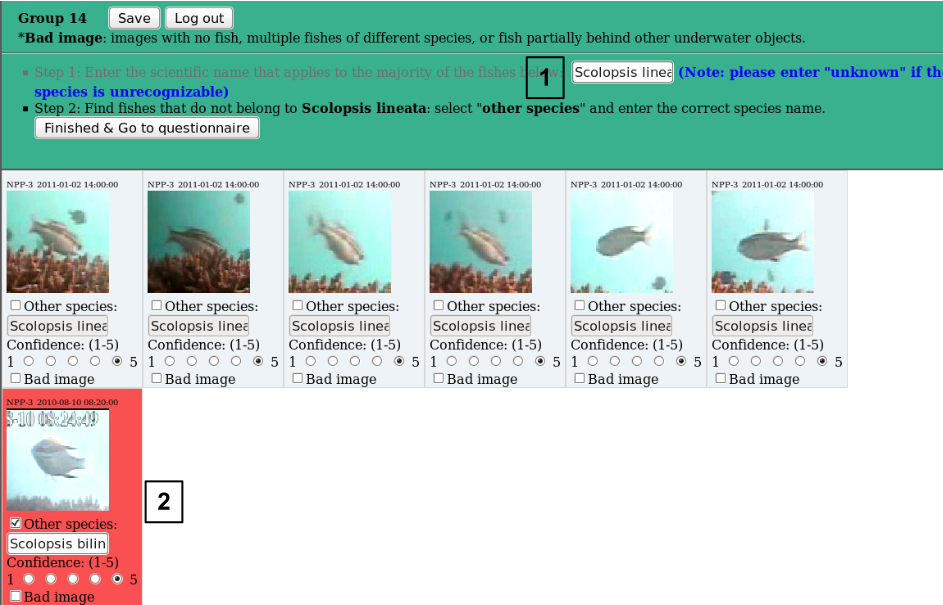
\includegraphics[width=0.48\textwidth]{expert_anno}
\caption{Expert labeling interface. (1): entering species name for the cluster; (2): correct individual species names.}%(1): entering the species name that applies to the majority of the images within the clusters; 
%(2): correcting individual species names for images that do not belong to the cluster.}
\label{fig:expert}
\end{figure}
%
\begin{figure*}[t!]
\centering
\subfigure[Labeling interface for non-expert players]{
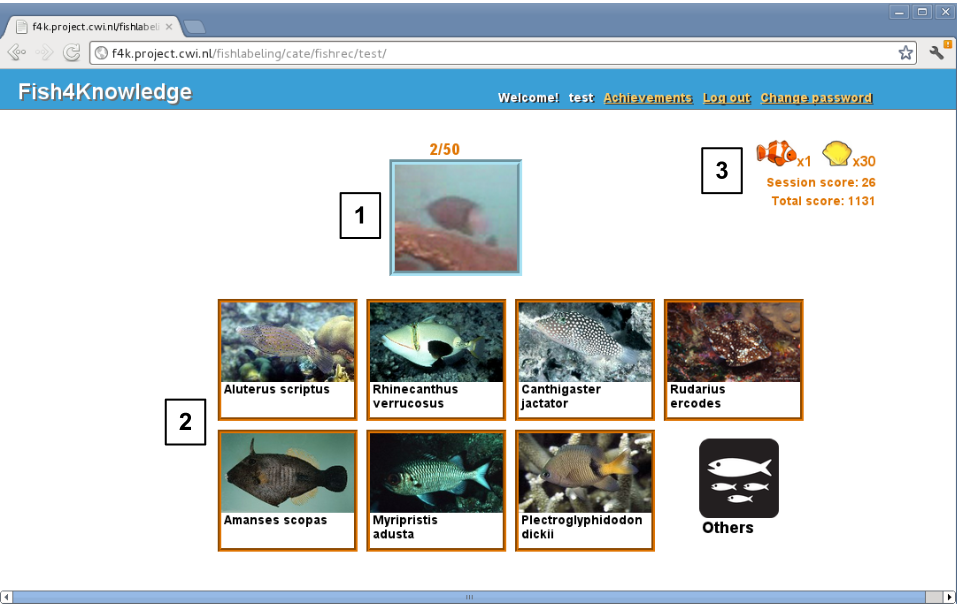
\includegraphics[width=0.48\textwidth, height=0.25\textwidth]{labeling_ui.png}
\label{fig:label_ui}
}
\subfigure[Achievment summary]{
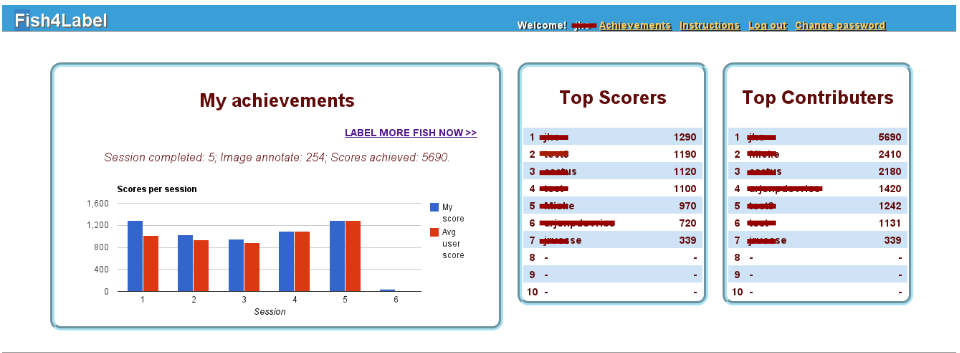
\includegraphics[width=0.48\textwidth, height=0.25\textwidth]{achieve_anon.png}
\label{fig:achieve_ui}
}
\caption{Non-expert labeling game interface. (1): query image; (2): candidate images; (3): feedback scores.}
\label{fig:nonexpert}
\end{figure*}
%
The expert labeling interface is used to assist experts (e.g., marine biologists, 
coral reef specialists, frequent divers) to create ground truth labels. 
These labels, while often small in quantity, are assumed to be of high quality.
They are considered a gold standard, e.g., for assessing the quality of non-expert
labels, and serve as feedback for non-experts so that they may learn 
and improve. 

%e.g., for assessing the quality of non-expert labels and 
%helping non-expert to learn and improve their label quality by providing 
%providing non-experts
%with feedbacks of their labels as training material. 

As pre-processing, the set of images that needs to be labeled is clustered (manually or with automatic clustering algorithms, e.g., ~\cite{boom12:supp}). 
At each screen, images within a cluster are presented to the expert user. 
See Fig.~\ref{fig:expert}. 
%
The labeling process consists of two steps. \\
\textbf{Step 1}: The user is asked to enter a species name that would apply to the majority of 
the images within the cluster. Once the name is entered, all images within the clusters are 
assigned the same name. \\
\textbf{Step 2}: When there exist images that do not belong to the same cluster, i.e., %there are 
images assigned a wrong species names after step 1, the user can select that ``wrong" image, and correct
its species name. 

In the worst case,  the expert users would manually enter the species name for each image when 
each single image within a cluster belongs to a different species. 
In the best case, when the cluster is pure, they only need to enter the label once for a cluster. 
Users can further indicate 1) their confidence in the labels they have entered, and
2) ``bad images", i.e., images that contain no fish, half fish or multiple fish.
As our images are extracted from video footage using automatic fish detection algorithms, 
the above ``bad images" may occur due to detection errors. 

\subsection*{Non-expert gaming interface}
The gaming interface is used to collect labels from laymen players. 
These labels are often large in quantity but noisy, 
therefore each image is labeled multiple times by multiple players. 
Post-processing is needed to aggregate the obtained labels into a final label. 

On the labeling screen, a \emph{query image} (image to be labeled) and a set of \emph{candidate images} (potential labels) 
are presented to the players. See Fig.~\ref{fig:label_ui}. 
%
The players are asked to compare the query image to the candidate images. 
They select one of the candidates if they believe
this candidate image should belong to the same species as the fish in the query image. 
If none of the candidates is similar enough to the query image, the ``others"  icon should be selected.

Each image to be labeled is assigned a priority score. 
In a default setting, if an image has been assigned many labels, then it has less priority
than images that have received no or very few labels. 
For instance, in the beginning all images are assigned a score of 1, 
and are updated as the labeling process goes on, computed as 1 divided by the number of labels it has received. 

Candidate images are prototype images of different species obtained from Fishbase~\cite{fisbase}. %\footnote{\url{http://www.fishbase.org}}.
To avoid overloading players with too many candidates, only 7 candidate images are shown for a query image. 
Candidate images are selected based on their similarity to the query image.
Different similarity measures can be applied; similarity scores are pre-computed and stored
in the back-end database when deploying the system. 

For each click, a feedback score is shown to the user. 
We consider two types of feedback scores: (1) expert feedback, computed as
the percentage of expert labels that agree with the chosen label,  if available; 
and (2) peer-agreement,  computed as the percentage of players' labels that agree
with the chosen label. 
%
Notice that with peer-agreement, the feedback score of a same $\{\text{image}, \text{label}\}$ pair may change
as more people play the game. In particular, when there are very few labels the scores are sensitive to erroneous decisions made by individual players, 
and these scores are likely to introduce bias to players' decisions. 
%
To handle this situation, for initial runs, labels generated by automatic methods or manual runs without feedback 
are used. 
%
%either manual runs or labels generated by automatic method, no feedback based
%on peer-agreement is given. 

Within the system, different methods of computing image priority, candidate similarity, 
and feedback scores can be easily extended and deployed. 

%achievements
Players can view their ``achievements" in the achievement screen (Fig.~\ref{fig:achieve_ui}). 
We show three types of statistics:
(i) achievements of the current user, including the number of sessions they have played, the number of images
they have labeled, as well as their per-session scores compared to that of the average scores achieved by other players; 
(ii) top scorers: the top 10 players in terms of the highest single session scores they have achieved;
and (iii) top contributors: the top 10 players in terms of the cumulative scores they have achieved. 
These scores are displayed in order to encourage users to aim for higher scores and play more sessions.

Table~\ref{tab:comp} shows a comparison between the resources used by experts and 
non-experts in the two labeling settings. In~\cite{jhe13:crowd} we report studies on user behavior with respect to 
our labeling system. 
%
\begin{table}[t!]
\caption{A comparison of resources used by experts and non-expert players during fish labeling.}
\begin{tabular}{lll}
\hline
Type & Candidates source &  Verification source \\
\hline
Experts  &  From their knowledge & Textbook\\
Non-experts & Given by the system & System feedback \\
\hline
\end{tabular}
\label{tab:comp}
\end{table}








\ifanon
\else
\section*{Acknowledgements}
This research was funded by European Commission FP7 grant 257024, in the Fish4Knowledge project (www.fish4knowledge.eu).
\fi

\renewcommand{\bibsection}{\section{\mbox{References}}}
\setlength{\bibsep}{1pt}
\bibliographystyle{abbrvnat}
%\footnotesize
\bibliography{oair2013-crowdsourcing}

\end{document}

%
%\cite{Giro2012:multi, Moeh2012:effe}.  Examples of crowdsourcing such
%ground truth collection in order to obtain larger scale datasets
%include  \cite{Russell08:Label} for image and video labeling or
%\cite{Hoss12:aggr} for INEX document/topic relevance assessments.
%
%Crowd-sourcing as a collaborative problem solving strategy has
%received much attention recently,
%
%In particular, within the IR and CV communities, where large scale
%ground truth data are needed, the wisdom of the crowd was shown to
%and are shown to provide effective solutions in a wide range of problems, 
%ranging from image/video annotation~\cite{Russell08:Label, Yuen09:Label, ahnl:04,
%anhl06:impr, ahnl06:peekaboom, Chen:2011:LFA}, 
%to text
%annotation~\cite{AMBATI10.244, Finin:2010:ANE} and search result
%assessments~\cite{eickhoff12:qual, Hoss12:aggr}. %kazai:overview11
%
%
%Creating such ground truth data sets typically requires a large
%amount of manual effort.  
%Crowd-sourcing is a commonly applied strategy. 

Social tagging is another related field where the crowd is used to tag images, including Flickr images~\cite{sigurbjornsson2008flickr}, 
museum art collections~\cite{trant2006exploring}. 
A number of studies has examined the quality or conditions of annotators. 
~\citet{theodosiou2011evaluating} studied the how the crowd can be conditioned to produce better results. 
~\citet{Kazai:2012:ASJ} and~\citet{Bailey08relevanceassessment} show that in information retrieval experts' judgement 
can not be replaced by novices. 
%
Among these studies, none of the tasks requires the type of expert knowledge as required in our task. 
That is, highly localized and domain specific knowledge. 
%
Further, in contrary to~\citet{Kazai:2012:ASJ} and ~\citet{Bailey08relevanceassessment} where the task setup is the same
for experts and non-experts, we study whether experts can be replaced by non-experts if we convert the task, i.e., 
converting the task from a ``non-expert mission-impossible" to ``a non-expert friendly" task. 


%
Another line of research focuses on aggregating and exploiting noisy annotations collected
via crowd-soucing. %within the context of active learning and result aggregating~\cite{Snow:2008}.
For instance, %in the field of NLP, 
\citet{Snow:2008} used a voting model to aggregate annotations
and proposed a bias correction approach to estimate the weights of non-expert annotators' annotation. 
%
\citet{AMBATI10.244} proposed an active learning
approach to machine translation that ``actively'' select next task based on collected annotations. 
\citet{Welinder:2010oc} proposed an online learning approach to dynamically select
annotators and the number of images assigned to annotators. 
Graphical models were used to aggregate judgements in~\cite{Hoss12:aggr}
and were used in~\cite{Welinder:2010fk} to model the annotation process
aimed at capturing multiple factors that has an impact on the 
annotators' judgement. 
%
While these are not the focus of our current study, 
we expect that they are relevant for applying
our approaches in practice, and our current study provides insights of where and when 
these approaches may be needed within our context.

%we aim to tackle an image recognition  
%task that requires extensive expert knowledge in marine biology with laymen's contributions. 
%%our task of species recognition for fish images is not trivial even for marine biologists. 
%%
%%We convert this problem to an image matching game and hypothesize that the expert  
%%recognition task can be solved simply by visual similarity assessment, and conduct a user 
%%study to examine whether this strategy leads to a promising solution.


%In the game, players are shown a single
%\emph{query image} along with multiple labeled images of candidate
%species, referred to as \emph{candidate labels}, and are asked to
%assign the query image to the label that depicts the same species as
%the fish in the image. 



%Much research in crowd-sourcing has been focused on the design of Human Intelligence 
%Tasks (HITs)~\cite{ahnl:04, anhl06:impr, ahnl06:peekaboom, eickhoff12:qual, Kazai09onthe, Kazai11crowd}. 
%%which includes aspects such as incentives, fesibility and quality control.
%Indeed, in order to generate useful results, the designed task should
%make workers~\emph{want to} as well as~\emph{able to} generate outputs.
%%and is capable to control over the quality of the submitted jobs.
%
%%Tasks such as image/video annotations or relevance assessments are
%%in general tedious work. 
%In order to solve the \emph{want to} problem, incentive is the key.
%%is an important aspect of the task design.
%A commonly used incentive is money, with advantages such as  
%being universal, easy to measure and flexible to be adjusted
%for balancing cost-profit~\cite{Horton:2010}. 
%%
%An important alternative is entertainment, i.e., the 
%so-called game with a purpose~\cite{ahnl08:desi}. 
%%
%A prime example of gamifying an annotation task is Luis von Ahn's ESP 
%game \cite{ahnl:04}. 
%%They posit that if the labeling game is entertaining enough so that 
%%people would play it as often as other online games, 
%%most of the Web images can be labelled by the players within a few months.
%%
%Within the image annotation context, similar games include Phetch~\cite{anhl06:impr}, 
%an online game that annotates images with explanatory text, Peekaboom~\cite{ahnl06:peekaboom}
%that locates objects in images. 
%%
%Different from our task, these games all target at general image annotation problems
%that do not require expert knowledge in specific domains.
%%
%Recently, \citet{eickhoff12:qual} showed quantitative and qualitative advantages of 
%using their GeAnn game to collect relevance assessments for search results. %TREC document/topic pairs.
%%
%%They demonstrated the generalisability of their game approach that it can be easily-transformed
%%solve to a image matching problem.
%%by developing a version for image from our project.  
%In this paper, we test the quality of data collected by a game that was inspired by GeAnn
%under a controlled experimental setup.
%
%
%
%While most of the studies so far focuses on the~\emph{want to} problem, 
%our primary focus is on the~\emph{able to} problem.
%%
%A smart way of presenting a problem %or decomposing a complicated problem into simpler sub-problems 
%may greatly reduce its difficulty and makes an infeasible task become feasible. 
%For example,  Foldit\cite{cooper2010:pred}
%uses a puzzle solving game for protein structure prediction.
%Their results show that it is possible to use non-experts to solve complicated
%scientific problems.
%Another example is Galaxy zoo~\cite{website:Galaxyzoo}, where citizens' wisdom
%contributes to morphological classification of galaxies.
%%
%Similar to these problems, we aim to tackle an image recognition  
%task that requires extensive expert knowledge in marine biology with laymen's contributions. 
%%our task of species recognition for fish images is not trivial even for marine biologists. 
%%
%%We convert this problem to an image matching game and hypothesize that the expert  
%%recognition task can be solved simply by visual similarity assessment, and conduct a user 
%%study to examine whether this strategy leads to a promising solution.
%%
%
%%\todo{About expert vs. non-expert, say that we are addressing a different problem, refer to comparison table of expert-non-expert actives}
%%\todo{
%%discuss crowdMM workshop '12~\cite{chen2012acm}
%%discuss conditioning of users with a database schema~\cite{theodosiou2011evaluating}
%%discuss impact of social tagging on Flickr tag recommendation~\cite{sigurbjornsson2008flickr}
%%discuss tag agreement of users in taggin museum art collections~\cite{trant2006exploring}
%%}

